% -----------------------------------------------------------------------------
% Thin wrapper preamble for Grad-IO slides
% Usage:
%  - Optionally set \def\beamerclassoptions{[<opts>]} before \input-ing this file
%    so a slide can control per-file beamer options (e.g. [handout,aspectratio=169]).
%  - This file ONLY issues the \documentclass once (honoring \beamerclassoptions)
%    and then loads the shared package `gradio-preamble.sty` which contains the
%    guarded package loads and macro definitions.
% -----------------------------------------------------------------------------
\ifdefined\beamerclassoptions
        % Expand \beamerclassoptions (which should be like "[notes=show]") safely
        \begingroup\edef\x{\endgroup\noexpand\documentclass\beamerclassoptions{beamer}}\x
\else
        \documentclass[handout,10pt,aspectratio=169]{beamer}
\fi

% Load the canonical shared preamble package. Try the local resources folder first
% so slide-level inputs continue to work in-place; if installed system-wide then
% \RequirePackage will also find it by name.
\IfFileExists{./gradio-preamble.sty}{\RequirePackage{./gradio-preamble}}{%
    \IfFileExists{gradio-preamble.sty}{\RequirePackage{gradio-preamble}}{%
        \RequirePackage{gradio-preamble}% final fallback to system-installed package
    }
}

% Any slide-specific packages or macros should be declared in the slide file
% after `% -----------------------------------------------------------------------------
% Thin wrapper preamble for Grad-IO slides
% Usage:
%  - Optionally set \def\beamerclassoptions{[<opts>]} before \input-ing this file
%    so a slide can control per-file beamer options (e.g. [handout,aspectratio=169]).
%  - This file ONLY issues the \documentclass once (honoring \beamerclassoptions)
%    and then loads the shared package `gradio-preamble.sty` which contains the
%    guarded package loads and macro definitions.
% -----------------------------------------------------------------------------
\ifdefined\beamerclassoptions
        % Expand \beamerclassoptions (which should be like "[notes=show]") safely
        \begingroup\edef\x{\endgroup\noexpand\documentclass\beamerclassoptions{beamer}}\x
\else
        \documentclass[handout,10pt,aspectratio=169]{beamer}
\fi

% Load the canonical shared preamble package. Try the local resources folder first
% so slide-level inputs continue to work in-place; if installed system-wide then
% \RequirePackage will also find it by name.
\IfFileExists{./gradio-preamble.sty}{\RequirePackage{./gradio-preamble}}{%
    \IfFileExists{gradio-preamble.sty}{\RequirePackage{gradio-preamble}}{%
        \RequirePackage{gradio-preamble}% final fallback to system-installed package
    }
}

% Any slide-specific packages or macros should be declared in the slide file
% after `% -----------------------------------------------------------------------------
% Thin wrapper preamble for Grad-IO slides
% Usage:
%  - Optionally set \def\beamerclassoptions{[<opts>]} before \input-ing this file
%    so a slide can control per-file beamer options (e.g. [handout,aspectratio=169]).
%  - This file ONLY issues the \documentclass once (honoring \beamerclassoptions)
%    and then loads the shared package `gradio-preamble.sty` which contains the
%    guarded package loads and macro definitions.
% -----------------------------------------------------------------------------
\ifdefined\beamerclassoptions
        % Expand \beamerclassoptions (which should be like "[notes=show]") safely
        \begingroup\edef\x{\endgroup\noexpand\documentclass\beamerclassoptions{beamer}}\x
\else
        \documentclass[handout,10pt,aspectratio=169]{beamer}
\fi

% Load the canonical shared preamble package. Try the local resources folder first
% so slide-level inputs continue to work in-place; if installed system-wide then
% \RequirePackage will also find it by name.
\IfFileExists{./gradio-preamble.sty}{\RequirePackage{./gradio-preamble}}{%
    \IfFileExists{gradio-preamble.sty}{\RequirePackage{gradio-preamble}}{%
        \RequirePackage{gradio-preamble}% final fallback to system-installed package
    }
}

% Any slide-specific packages or macros should be declared in the slide file
% after `\input{.../resources/preamble.tex}`.

`.

`.




\begin{document}
\title{Extensions and Variants}
\author{Chris Conlon}
\institute{Grad IO}
\date{\today}

\frame{\titlepage}

\subsection*{Micro-Moments and Demographics}
\begin{frame}
\frametitle{BLP Extensions: Demographics (Nevo 2000)}
\begin{itemize}
\item It is helpful to allow for interactions with consumer demographics (such as income).
\item A few ways to do this:
\begin{itemize}
\item You could just use cross sectional variation in $s_{jt}$ and $\overline{y}_t$ (mean or median income).
\item Better: Divide up your data into additional ``markets'' by demographics: do you observe $\mathfrak{s}_{jt}$ at this level? [May not be possible!]
\item Better: Draw $y_{it}$ from a geographic specific income distribution. Draw $\nu_i$ from a general distribution of unobserved heterogeneity.
\end{itemize}
\item Ex: Nevo (2000) Cereal demand sampled individual level $y_{it}$ from geographic specific CPS data
\item Joint distribution of income, income-squared, age, child at home.
\begin{align*}
\beta_i = \overline{\beta} + \Pi y_i + \Sigma \nu_i
\end{align*}
\end{itemize}
\end{frame}

\begin{frame}
\frametitle{BLP Extensions: Panel Data (Nevo 2000)}
\begin{itemize}
\item with enough observations on the same product it is possible to include fixed effects
\begin{eqnarray*}
\delta_{jt}(\widetilde{\theta}_2) = x_{jt} \beta - \alpha p_{jt} + \underbrace{\xi_{jt}}_{\xi_{j} + \xi_t + \Delta \xi_{jt}}
\end{eqnarray*}
\item What does $\xi_{j}$ mean in this context?
\item What would $\xi_t$ mean in this context?
\item $\Delta \xi_{jt}$ is now the structural error term, this changes our identification strategy a little.
\item We need instruments that change \alert{within product and across market}.
\begin{itemize}
\item ie: $z_{jt} - \overline{z}_{\cdot t} - \overline{z}_{j \cdot } = \Delta z_{jt}$ has to have some variation left!
\end{itemize}
\end{itemize}
\end{frame}


\begin{frame}
\frametitle{Extensions: Micro Data (Petrin 2002), (microBLP 2004)}
Suppose we had additional data on behavior of individuals (in addition to aggregate market shares).
\begin{itemize}
\item Examples:
\begin{itemize}
\item For some customers have answer to ``Which car would you have purchased if the car you bought was not available?''
\item Demographic data on purchasers of a single brand.
\item Full individual demographic and choice data.
\end{itemize}
\end{itemize}
\end{frame}

\begin{frame}
\frametitle{Extensions: Micro Data: Nielsen Panelists}
Nielsen data surveys panelists on everything they buy with a UPC code including what store they purchased from.
\begin{itemize}
\item Also tracks household characteristics (Race, Income, Education, HH Size, etc.)
\item Can calculate covariance of characteristics (such as price) with demographics (income, education, etc.) \alert{conditional on purchase}
\item Can calculate purchase probability conditional on demographics: Did you buy any yogurt this trip, week, month, year?
\end{itemize}
Should we use these as individual data? Or Aggregate data from scanner data with additional moments?
\end{frame}

\begin{frame} \frametitle{Extensions: Micro Data (Petrin 2002), (microBLP 2004)}
\begin{itemize}
\item Previously we had moment conditions from orthogonality of structural error $(\xi)$ and $(X,Z)$ in order to form our GMM objective.
\begin{eqnarray*}
\mathbb{E}[\xi_{jt} | z_{jt}]=0 \rightarrow \mathbb{E}[\xi_{jt}' Z_{jt}]=0
\end{eqnarray*}
\item We can incorporate additional information using ``micro-moments'' or additional moment conditions to match the micro data.
\begin{itemize}
\item $Pr(\mbox{ i buys j } | y_i \in [0,\$20K])= c_1$ or  $Cov(d_i, s_{ijt}) = c_2$
\item Construct an additional error term $\zeta_1,\zeta_2$ and interact that with instruments to form additional moment conditions.
\item Econometrics get tricky when we have a different number of observations for $\mathbb{E}[\zeta'  Z_m]=0$ and  $\mathbb{E}[\xi'  Z_d]=0$.
\begin{itemize}
\item May not be able to get covariance of moments taken over different sets of observations!
\item People often assume optimal weight matrices are block diagonal.
\end{itemize}
\end{itemize}
\end{itemize}
\end{frame}



\begin{frame} \frametitle{Extensions: Complete Micro Data (Grieco, Murry, Pinkse, Sagl 2022)}
\footnotesize
\begin{align*}
(\hat{\beta}, \hat{\theta_2}, \hat{\delta})=\underset{\beta, \theta_2, \delta}{\arg \min }(\underbrace{-\log \hat{L}(\theta_2, \delta)+\hat{\Pi}(\beta, \delta)}_{\hat{\Omega}(\beta, \theta_2, \delta)})
\end{align*}
\begin{itemize}
\item $\log \hat{L}(\theta_2, \delta)$ is individual log-likelihood where $\delta_{jm}$ are free parameters and $\theta_2$ are nonlinear parameters.
\item $\hat{\Pi}(\beta,\delta)$ is derived from the moments: $\mathbb{E}[\left(\delta_{jm}-\beta x_{jm} - \alpha p_{jm}\right)\, z_{jm}]=0$
\item We don't impose $s_{jt} = \mathfrak{s}_{jt}$
\end{itemize}
Efficiency requires correcting micro-data to avoid double-counting:
\begin{align*}
\log \hat{L}(\theta, \delta)=\underbrace{\sum_{m=1}^M \sum_{j=0}^{J_m} \sum_{i=1}^{N_m} w_{i m} d_{i j m} \log s_{j m}(y_{i m})}_{\text {micro }}+\underbrace{\sum_{m=1}^M \sum_{j=0}^{J_m}\left(N_m s_{j m}-\sum_{i=1}^{N_m} w_{i m} d_{i j m}\right) \log s_{j m}}_{\text {macro }}
\end{align*}
\end{frame}

\begin{frame} \frametitle{Extensions: Second Choices (Conlon, Mortimer, Sarkis 2022)}
\small
We need to see at least some $\calD_{jk}$
\begin{align*}
\min_{s_{ij}, \pi_i}\sum_{(k,j) \in \text{OBS}} \left( \calD_{kj} - D_{kj}\right)^2+ & \lambda_1 \cdot  \sum_j \left(\calS_j - \sum_i \pi_i \cdot s_{ij} \right)^2\\ %+ \lambda_2 \norm{\pi_i}^2 \\
\text{subject to} \quad 
%\nonumber    s_j &= \sum_{i=1}^I \pi_i \cdot s_{ij}\\
\nonumber    D_{kj} &= \sum_{i=1}^I \pi_i \cdot \frac{s_{ij}}{1-s_{ik}} \cdot \frac{s_{ik}}{s_{k}}\\
\nonumber    \calS_j &= \frac{\mathcal{Q}_j }{\overline{q}_0 +\sum_{k \in \calJ_t} \mathcal{Q}_k}  \\
\nonumber   0\leq s_{ij}, \pi_i, s_j, D_{kj} \leq 1,& \quad
   \sum_{i=1}^I \pi_i = 1,\quad
   \sum_j s_{ij} = 1 
\end{align*}
\vspace{-.25cm}
\begin{itemize} 
  \item Semi-parametric (finite-mixture) if we let $I$ grow
\item Use cross validation to select \# of types $I$.
%\item With $\lambda_2 >0$ we penalize $HHI$ of $w_i$ and becomes \alert{elastic net} 
\end{itemize}
\end{frame}




\subsection*{Models without $\varepsilon$}


\begin{frame}
\frametitle{Alternative: Vertical Model (Bresnahan 1987)}
\footnotesize
\begin{itemize}
\item Imagine everyone agreed on the quality of the products offered for sale.
\item The only thing people disagree on is willingness to pay for quality
\begin{eqnarray*}
U_{ij} = \overline{u} + \delta_j - \alpha_i p_j
\end{eqnarray*}
\item How do we estimate?
\begin{itemize}
\item Sort goods from $p_1 < p_2  < p_3 \ldots < p_J$.\\
 It must be that $\delta_1 < \delta_2 < \ldots < \delta_J$. Why?
 \item Normalize o.g. to $0$ so that $ 0 > \delta_1 -\alpha_i p_1$ or $\alpha_i > \delta_1 / p_1$.
 \item $s_0 = F(\infty) - F(\frac{\delta_1}{p_1})  = 1 - F(\frac{\delta_1}{p_1}) $ where $F(\cdot)$ is CDF of $\alpha_i$.
 \item In general choose $j$ IFF:
 \begin{eqnarray*}
 \frac{\delta_{j+1} - \delta_j}{p_{j+1} -p_j} < \alpha_i < \frac{\delta_j  - \delta_{j-1}}{p_j - p_{j-1}}\\
 s_j = F\left(\frac{\delta_{j+1} - \delta_j}{p_{j+1} -p_j} \right) - F\left(\frac{\delta_j  - \delta_{j-1}}{p_j - p_{j-1}} \right)
 \end{eqnarray*}
\end{itemize}
\end{itemize}
\end{frame}

\begin{frame}
\frametitle{Alternative: Vertical Model (Bresnahan 1987)}
Estimation
\begin{itemize}
\item Choose parameters $\theta$ of $F(\cdot)$ in order to best match $s_j$.
\begin{itemize}
\item Can do MLE $\arg \max_{\theta} \sum_j -\mathfrak{s}_j \log s_{j}(\theta)$.
\item Can do least squares $\sum_j (\mathfrak{s}_j - s_{j}(\theta) )^2$.
\item Can do IV/GMM if I have an instrument for price.  $\delta_j = x_j \beta + \xi_j$.
\item Extremely easy when $F\sim \exp(\lambda)$.
\end{itemize}
\item What about elasticities?
\begin{itemize}
\item When I change the price of $j$ it can only affect $(s_{j-1},s_j, s_{j+1})$.
\item We have set all of the other cross-price elasticities to be zero.
\item If a luxury car and a truck have similar prices, this can create strange substitution patterns.
\end{itemize}
\end{itemize}
\end{frame}

\begin{frame} \frametitle{Pure Characteristics Model: Berry Pakes (2001/2007)}
\footnotesize
\begin{eqnarray*}
u_{ij} = \delta_j + \beta_i x_{jt} + \xi_{jt} + \underbrace{\sigma_e }_{\rightarrow 0} \cdot \varepsilon_{ijt}
\end{eqnarray*}
\begin{itemize}
\item Can think of this like random coefficients model where we take the variance of $\epsilon$ to zero.
\item Can think of this a vertical model, with vertical tastes over several characteristics.
\begin{itemize}
\item PCs: everyone prefers more Mhz, more RAM, and more storage but differ in WTP.
\item Possible that there is no PC specific $\varepsilon$.
\end{itemize}
\item Advantages
\begin{itemize}
\item Logit error means there is always some substitution to all other goods. 
\item Reality may be you only compete with a small number of competitors.
\item Allows for \alert{crowding} in the product space.
\end{itemize}
\item Disadvantage: no closed form for $s_j$, so estimation is extremely difficult.
\item Minjae Song (Homotopy) and Che-Lin Su (MPCC) have made progress using two different approaches.
\end{itemize}
\end{frame}


\subsection*{A Semiparametric Estimator}

\begin{frame}
\frametitle{Even More Flexibility (Fox, Kim, Ryan, Bajari)}
Suppose we wanted to nonparametrically estimate $f(\beta_i | \theta)$ instead of assuming that it is normal or log-normal.
\begin{eqnarray*}
s_{ij} &=& \int \frac{\exp[x_{j} \beta_i  ]}{1+\sum_k \exp[x_{k} \beta_i  ]} f(\beta_i | \theta)
\end{eqnarray*}
\begin{itemize}
\item Choose a distribution $g(\beta_i)$ that is more spread out that $f(\beta_i | \theta)$
\item Draw several $\beta_{s}$ from that distribution (maybe 500-1000).
\item Compute $\hat{s}_{ij}(\beta_s)$ for each draw of $\beta_s$ and each $j$.
\item Holding $\hat{s}_{ij}(\beta_s)$ fixed, look for $w_s$ that solve
\begin{eqnarray*}
\min_w \left(s_j -  \sum_{s=1}^{ns} w_s \hat{s}_{ij}(\beta_s) \right)^2 \quad \mbox{ s.t. } \sum_{s=1}^{ns} w_s = 1, \quad w_s \geq 0 \quad \forall s
\end{eqnarray*}
\end{itemize}
\end{frame}

\begin{frame}
\frametitle{Even More Flexibility (Fox, Kim, Ryan, Bajari)}
% Hey this is lasso
\begin{itemize}
\item Like other semi-/non- parametric estimators, when it works it is both flexible and very easy.
\item We are solving a least squares problem with constraints: positive coefficients, coefficients sum to 1.
\item It tends to produce \alert{sparse models} with only a small number of $\beta_s$ getting positive weights.
\begin{itemize}
\item Why? There is an $L_1$ penalty term (We are doing \alert{non negative LASSO}!)
\end{itemize}
\item This is way easier than solving a random coefficients logit model with all but the simplest distributions.
\item There is a bias-variance tradeoff in choosing $g(\beta_i)$.
\item Incorporating parameters that are not random coefficients loses some of the simplicity.
\item I have no idea how to do this with large numbers of fixed effects.
\end{itemize}
\end{frame}


\begin{frame}
\frametitle{Fully Nonparametric Demand (Compiani 2019)}
Takes identification arguments in Berry Haile (2014) to the data. Looks at a sieve approximation to
\begin{align*}
\sigma_{j}^{-1}(\calS_t,\widetilde{\theta}_2)
\end{align*}
Using the \alert{Bernstein Polynomials}
\begin{itemize}
\item Bernstein polynomials make it possible to enforce shape restrictions and \alert{monotonicity} which is important
\item Estimates demand for strawberries (organic vs. non-organic)
\item Suggests that both for markups and merger effects we don't have sufficiently flexible demand models.
\end{itemize}
\end{frame}


%
%\begin{frame}{Differentiation Instruments: Gandhi Houde (2016)}
%\begin{center}
%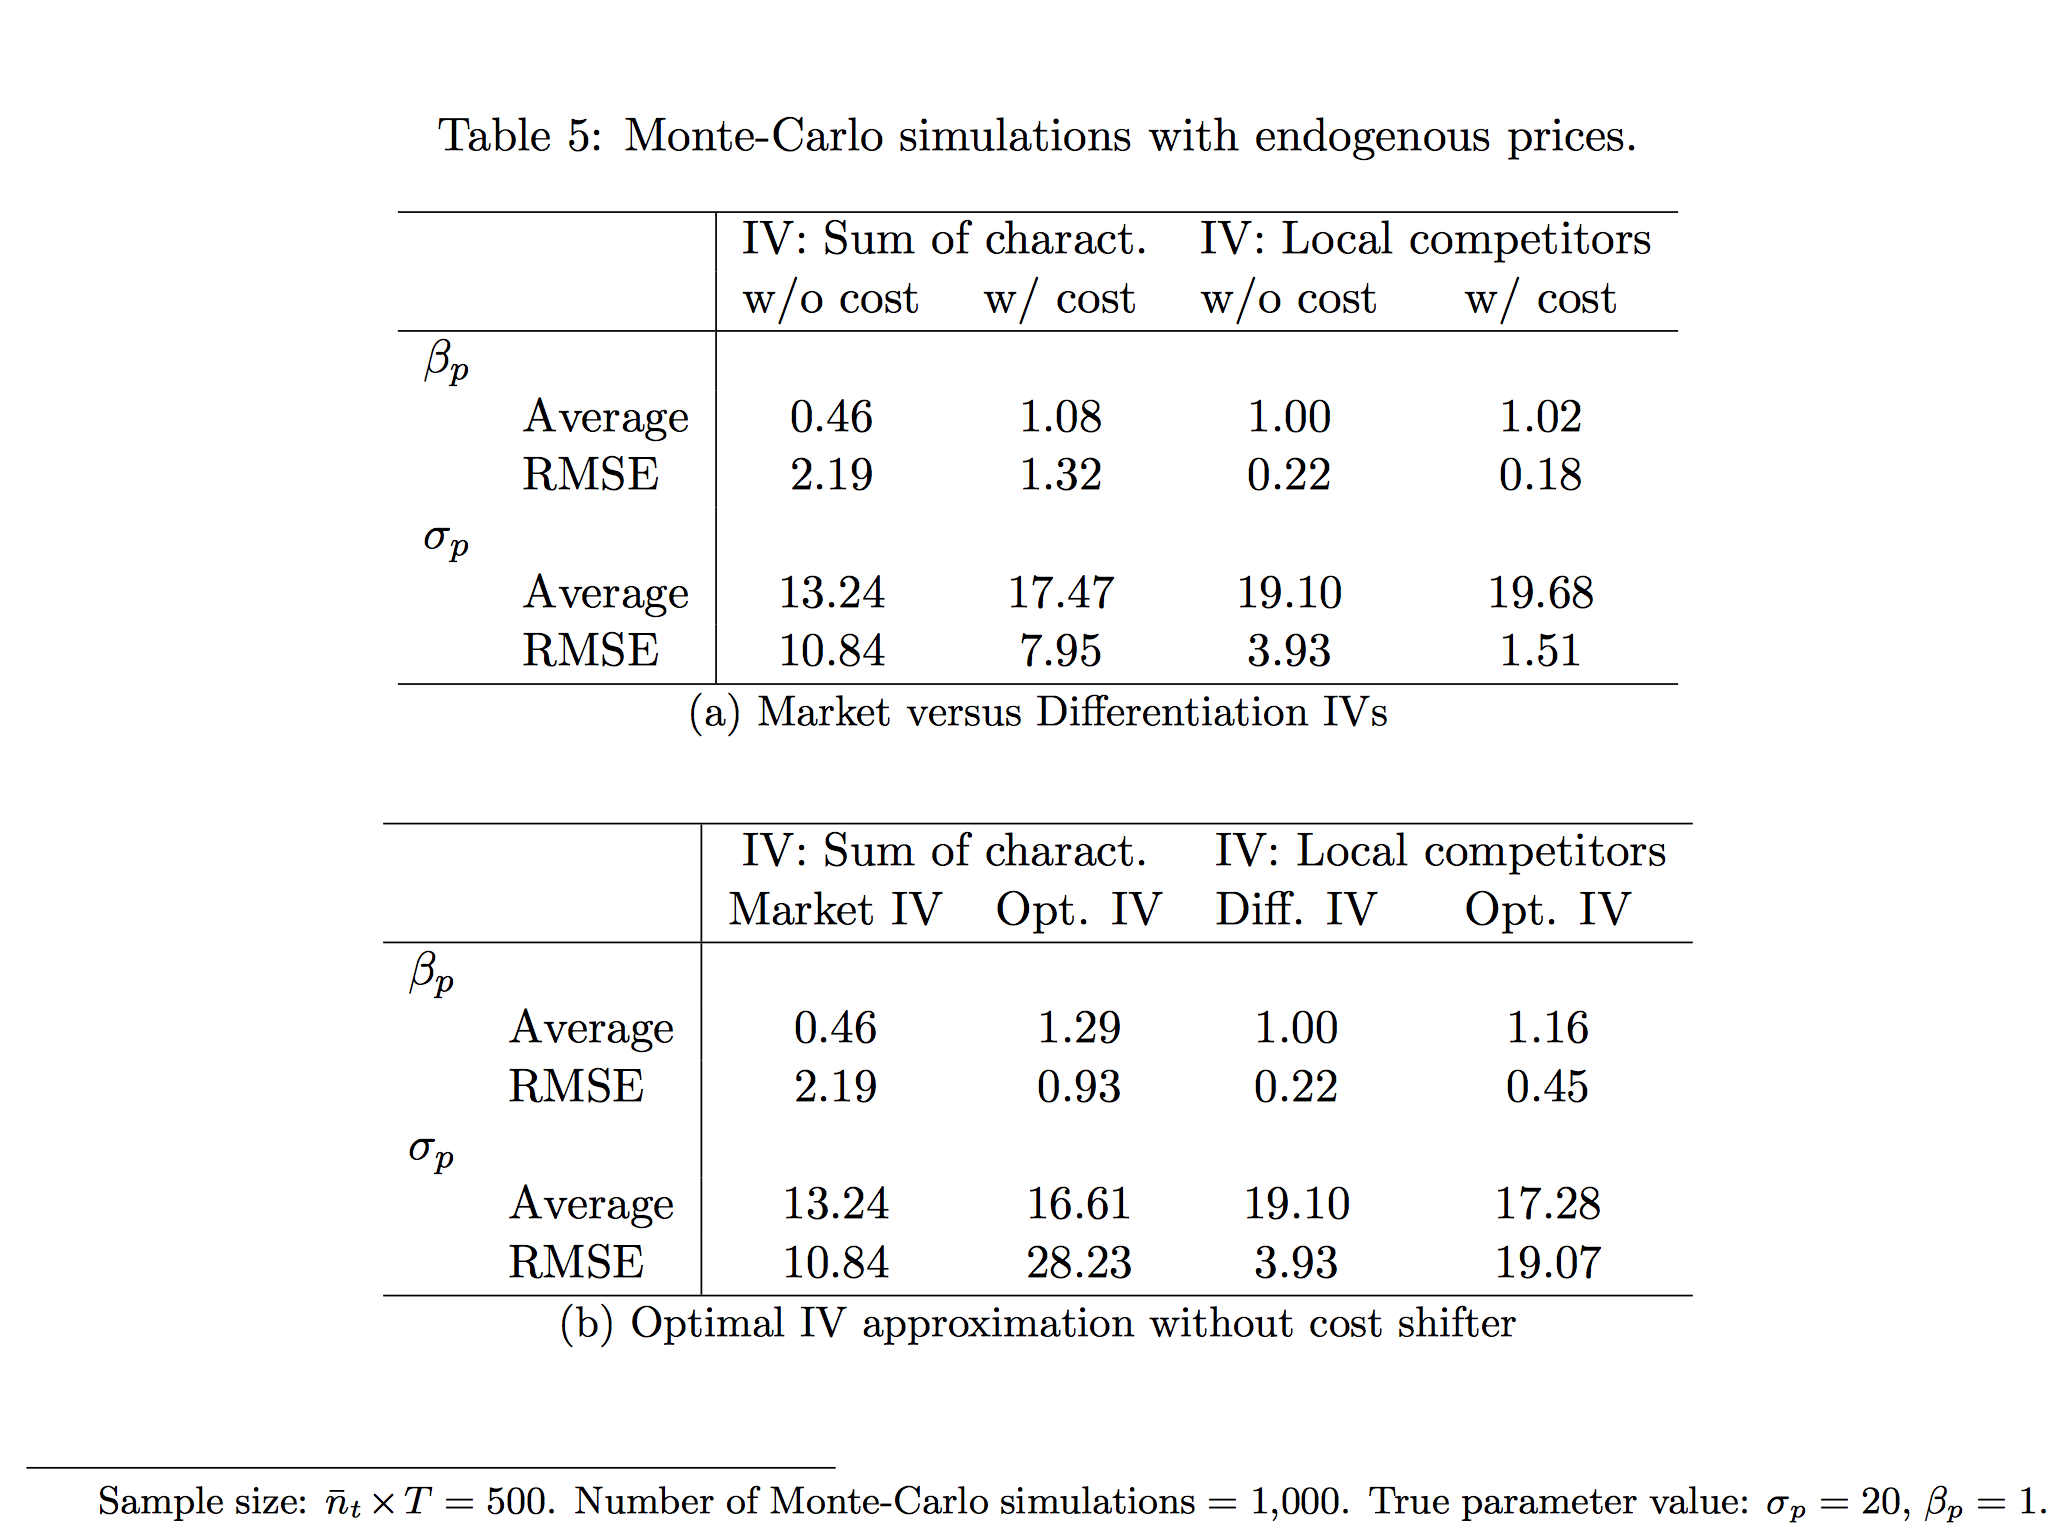
\includegraphics[width=3.8in]{resources/d_iv2.png}
%\end{center}
%\end{frame}
%



%
%\begin{frame} \frametitle{Extensions: Supply Moments}
%\begin{itemize}
%\item We can also impose the Bertrand FOC as a set of additional moments.
%\item First parametrize marginal cost
%\begin{eqnarray*}
%\ln mc_{jt} = \gamma_1 x_{jt} + \gamma_2 w_{jt} + \omega_{jt}
%\end{eqnarray*}
%\item helpful to constrain MC to be positive always.
%\item Note that for any vector of prices $p$ and demand parameters $\theta$ we can recover a unique vector of marginal costs (by solving the system of linear equations).
%\item Imposing the supply side only helps if we have information about the marginal costs / production function that we would like to impose
%\item Imposing these restrictions is helpful in constraining markups (so that implied MC are always positive, etc.).
%\item Misspecified functional forms for costs can cause problems!
%\end{itemize}
%\end{frame}





\end{document}